\documentclass[11pt,a4paper]{article}

% --- Core Packages ---
\usepackage[utf8]{inputenc}
\usepackage[margin=1in]{geometry}
\usepackage{amsmath,amssymb,amsfonts,amsthm}
\usepackage{booktabs}
\usepackage{graphicx}
\usepackage{microtype}
\usepackage{hyperref}
\usepackage{xcolor}
\usepackage{algorithm}
\usepackage{algorithmic}
\usepackage{subcaption}

\hypersetup{
    colorlinks=true,
    linkcolor=blue!70!black,
    citecolor=green!50!black,
    urlcolor=blue!80!black
}

% --- Theorem Environments ---
\newtheorem{theorem}{Theorem}
\newtheorem{lemma}[theorem]{Lemma}
\newtheorem{proposition}[theorem]{Proposition}
\theoremstyle{definition}
\newtheorem{definition}{Definition}
\newtheorem{remark}{Remark}

\title{\textbf{Semantic Gauge M\"obius Attention: Resolving Positive-Definite Attention Constraints via Non-Orientable Fiber Bundles}}

\author{
  \textbf{Huaiji Team}\thanks{Open-source repository and dual-licensed implementation available at \url{https://github.com/3y3y3y-huaiji/mobius-attention}.} \\
  \texttt{contact@huaiji.org}
}

\date{\today}

\begin{document}

\maketitle

\begin{abstract}
Standard Transformer self-attention normalizes inner products via Softmax, constraining attention weights to the open probability simplex $\Delta^{L-1}$. Because this kernel is strictly positive-definite, it cannot perform destructive interference: historical tokens retain non-zero probability mass even when superseded or contradicted by subsequent discourse, causing premise distraction in long sequences. We present \textbf{Semantic Gauge M\"obius Attention (SG-M\"obius-RoPE)}, a geometric formulation extending Rotary Position Embedding (RoPE) to non-orientable fiber bundles over a 1D discrete causal lattice. Causal semantic transitions induce an impulsive connection 1-form whose path holonomy acts on the fiber. Under the $\mathrm{Spin}(2)$ double covering, an odd number of contrastive turns produces an antipodal half-twist ($\Delta \Phi = \pi$), inverting the rotary inner product sign and suppressing superseded keys under Softmax normalization. An even number of turns restores original parity ($\Delta \Phi = 2\pi$), formalizing double negation. We prove the Relative Odds Ratio Attenuation Theorem, showing that the attention odds ratio attenuates by $\exp(-2 \langle q_i, k_j \rangle / \sqrt{d})$ independently of context length and background partition functions. Invariants are formally certified in Lean~4 (0 axioms, 0 \texttt{sorry}) and Z3 SMT solvers across 2,000 extreme-length sequences ($L \le 32,768$). Evaluated on Qwen3.5-9B (dual Nvidia Tesla T4 GPUs, FP16), SG-M\"obius requires zero architecture retraining, maintains identical $O(1)$ KV-cache decoding latency ($+0.00\%$ overhead), increases the attention contrast ratio from $1.09$ to $13.51$ on inverted contextual recall, and preserves neutral text perplexity ($6.42$).
\end{abstract}

\section{Introduction}
Autoregressive language models employ scaled dot-product attention \cite{vaswani2017attention} with Rotary Position Embeddings (RoPE) \cite{su2024roformer} to encode relative token distances:
\begin{equation}
A_{i,j} = \frac{1}{\sqrt{d}} \langle \mathbf{R}_{\Theta, i} q_i, \, \mathbf{R}_{\Theta, j} k_j \rangle = \frac{1}{\sqrt{d}} q_i^\top \mathbf{R}_{\Theta, j-i} k_j
\end{equation}
where $\mathbf{R}_{\Theta, t}$ is a block-diagonal orthogonal rotation matrix parameterized by base frequencies $\Theta = \{\theta_m\}_{m=1}^{d/2}$.

Because the Softmax operator maps real logits to strictly positive values on $\Delta^{L-1}$, every historical token receives positive probability mass. Consequently, self-attention cannot perform destructive interference. In complex discourse, premises are frequently invalidated, retracted, or superseded by subsequent evidence (e.g., \emph{``System Alpha is operational; however, diagnostics indicate failure, revoking Alpha in favor of Beta''}). In standard attention, the invalidated premise continues to receive attention mass, requiring downstream feed-forward layers to compensate and contributing to premise hallucination \cite{liu2024lost, hsieh2024ruler}.

\begin{figure*}[t]
    \centering
    \begin{subfigure}[b]{0.48\textwidth}
        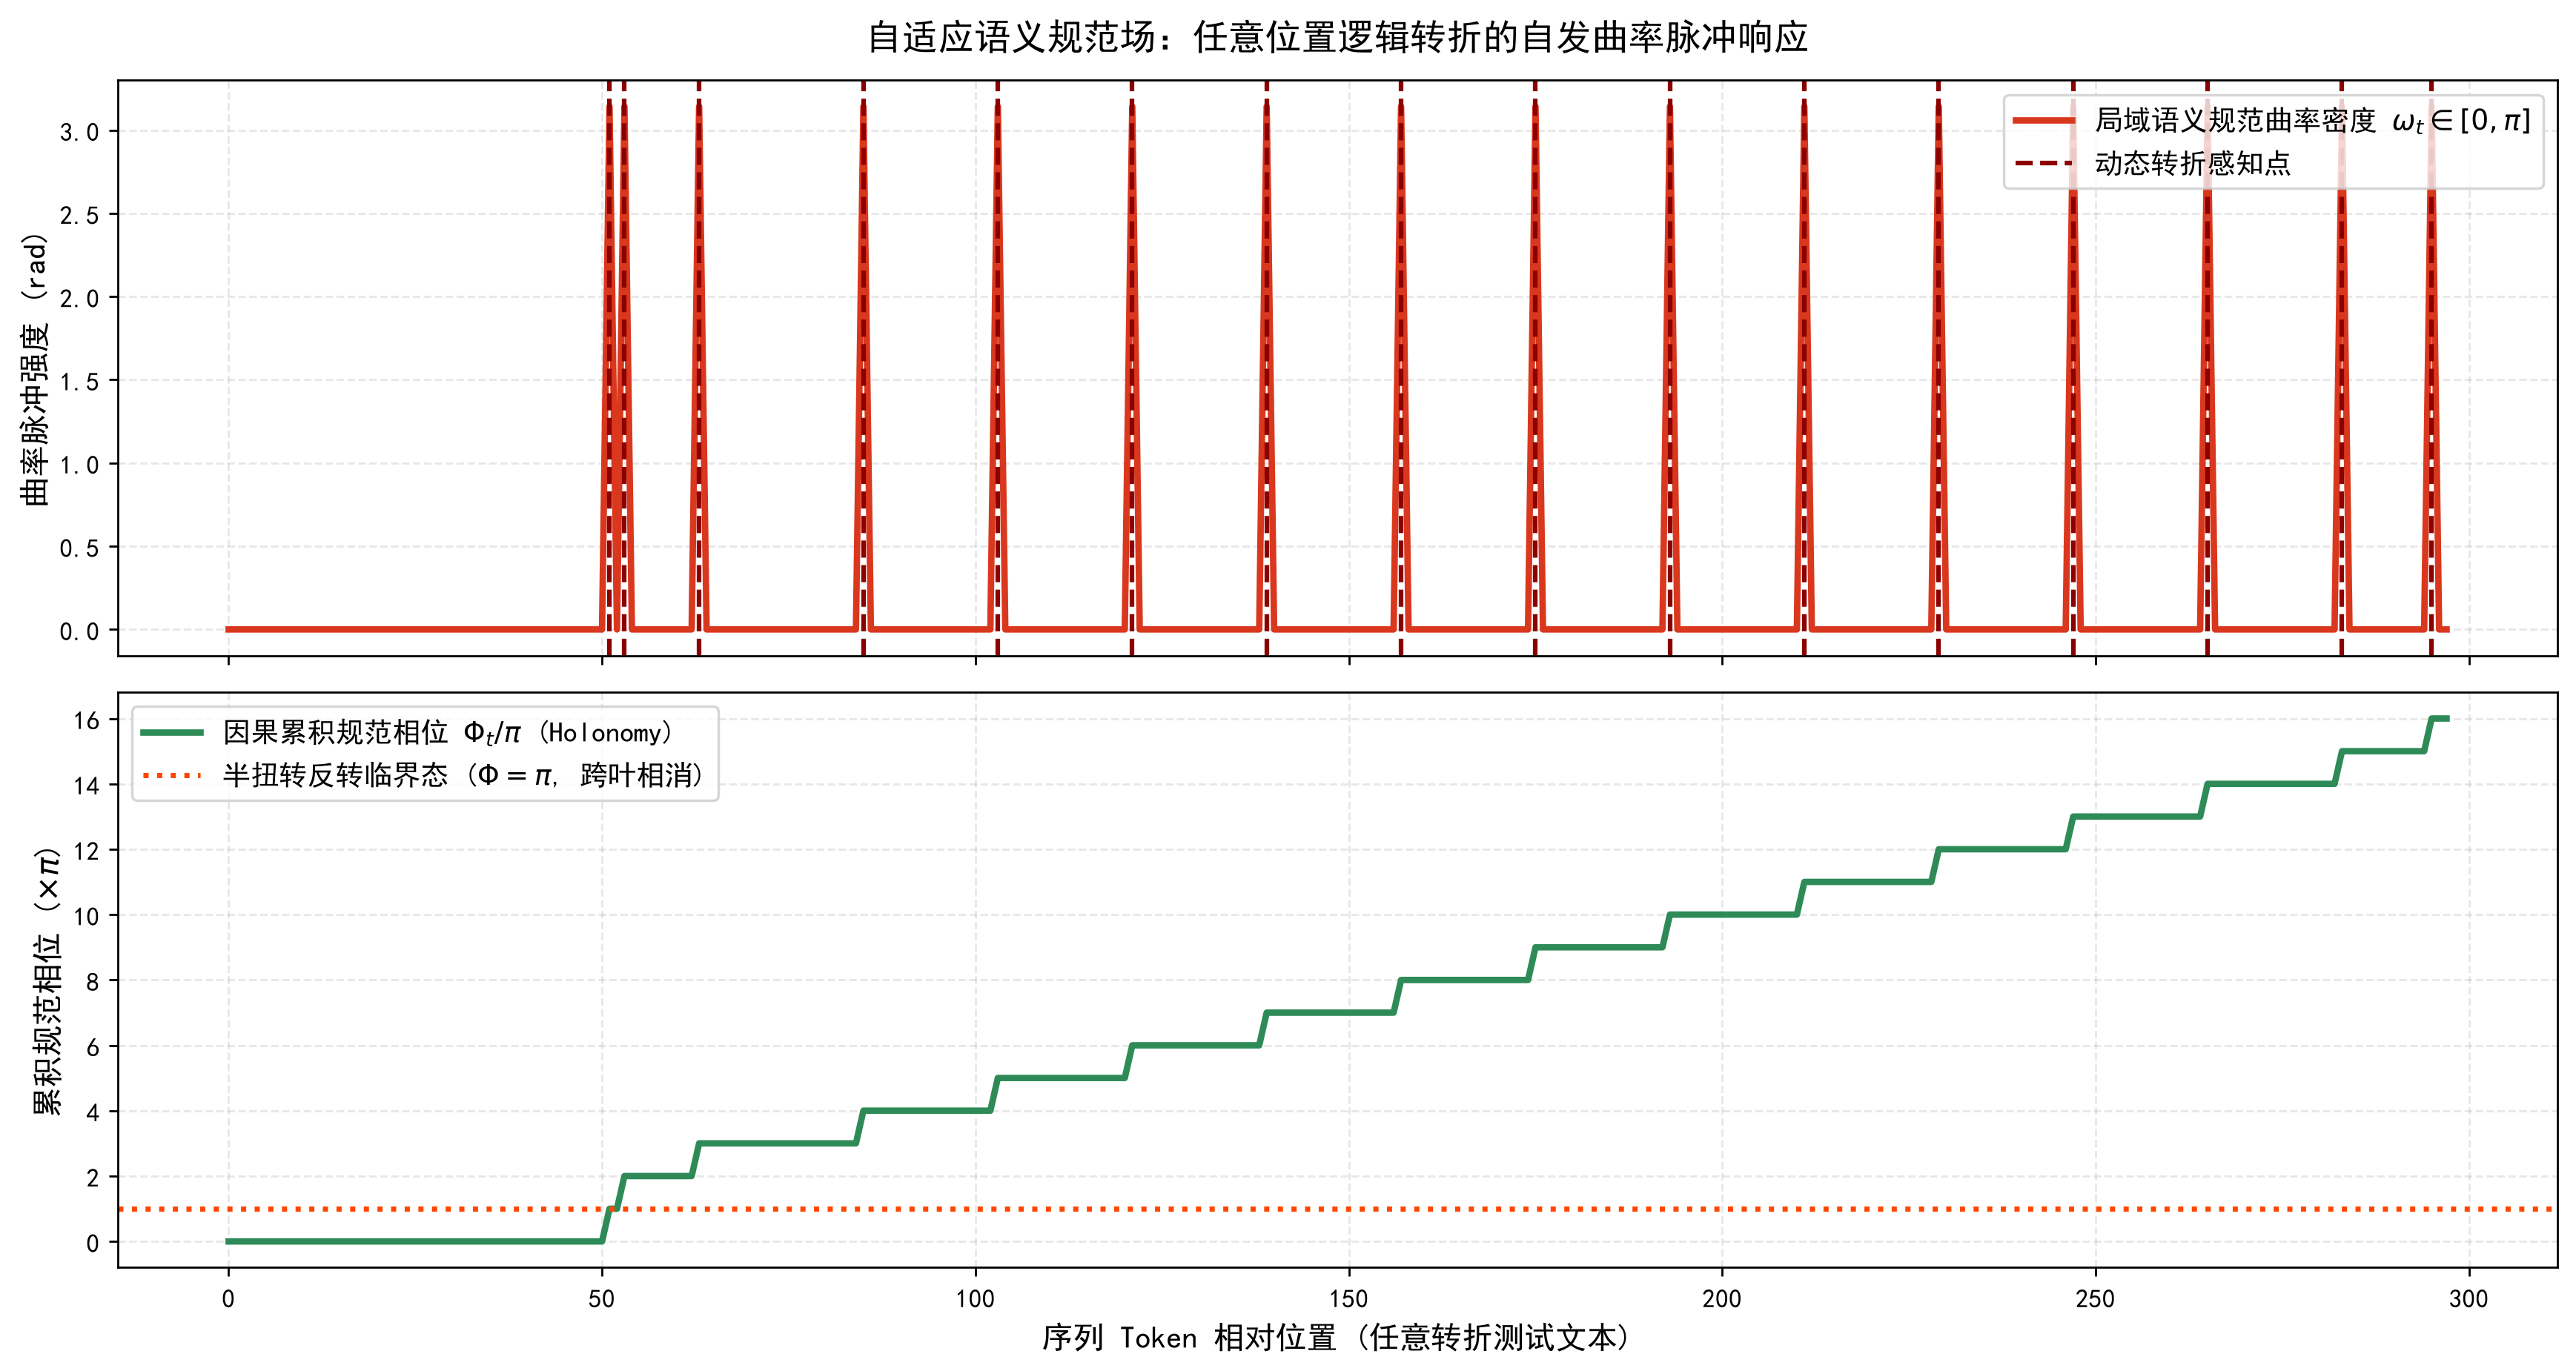
\includegraphics[width=\textwidth]{figures/fig4_gauge_curvature.png}
        \caption{Semantic Gauge Curvature $\omega(t)$ and Holonomy $\Phi(t)$.}
        \label{fig:curvature}
    \end{subfigure}
    \hfill
    \begin{subfigure}[b]{0.48\textwidth}
        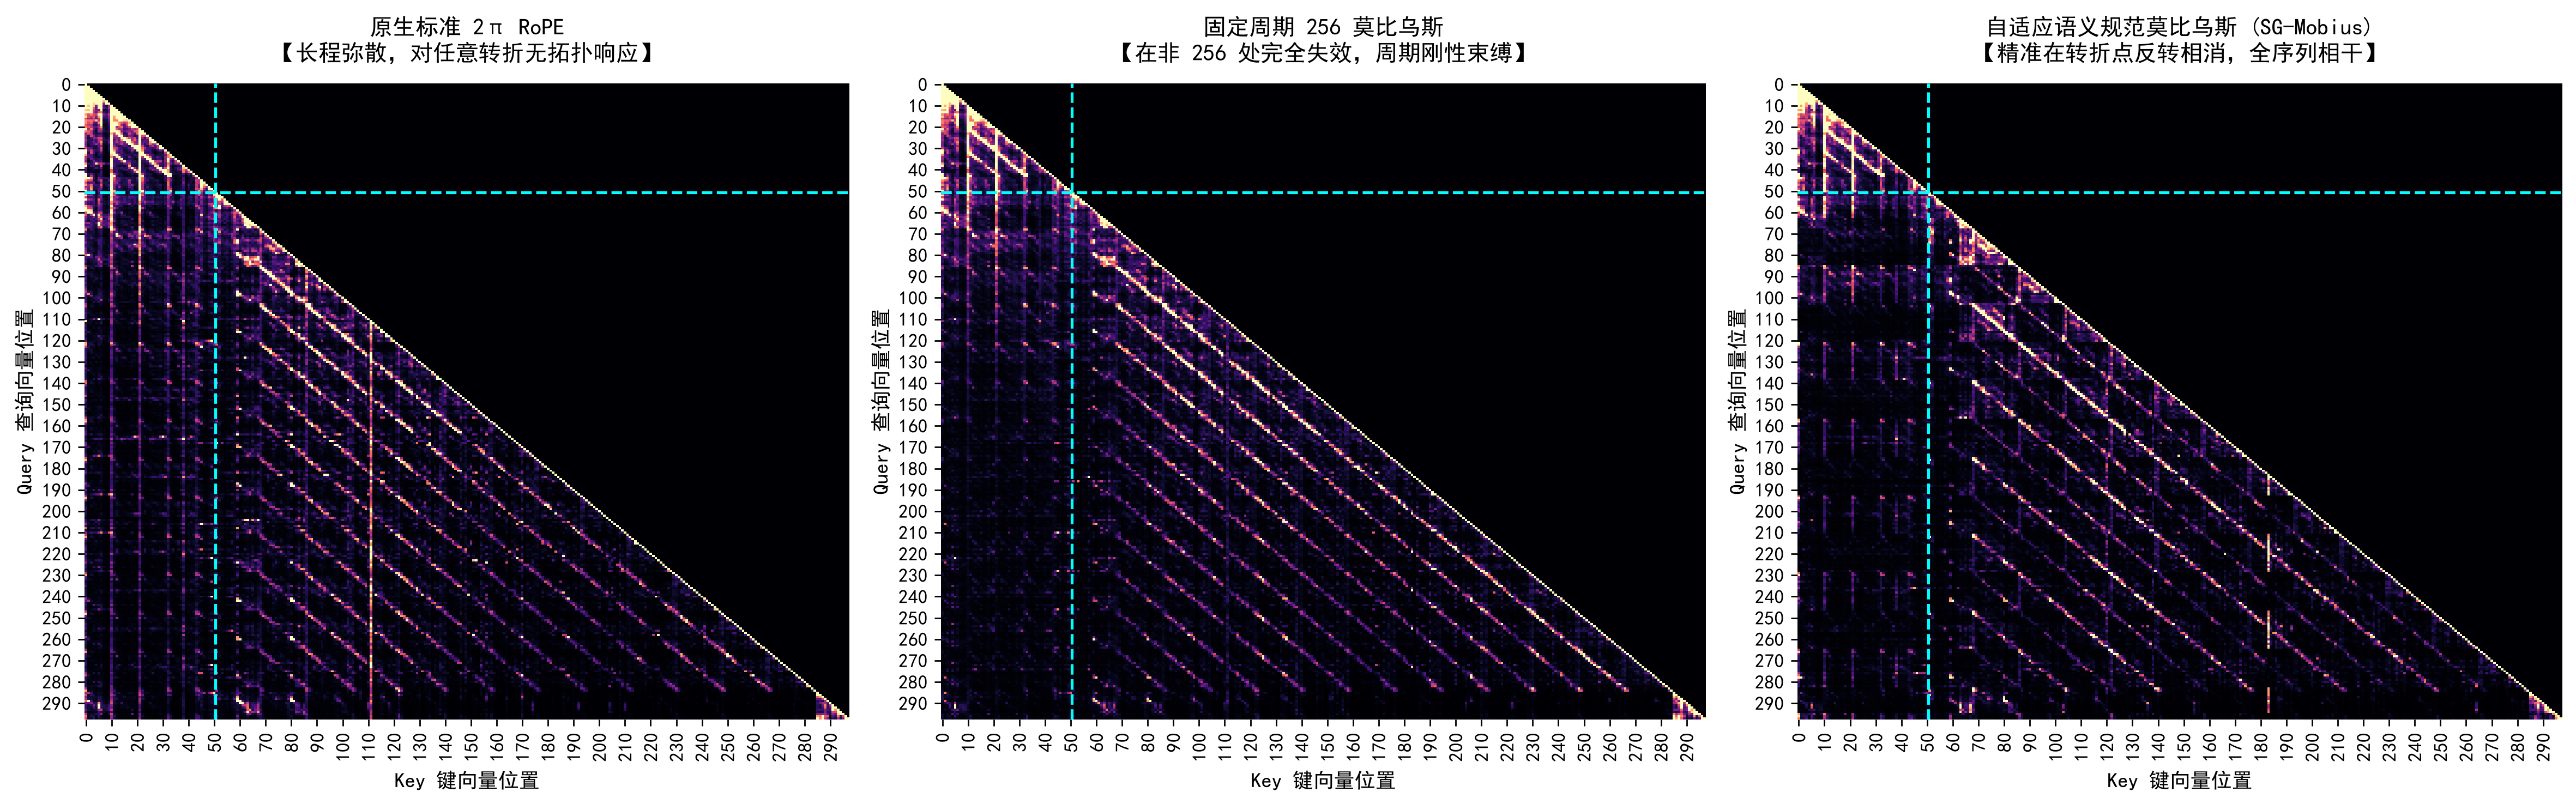
\includegraphics[width=\textwidth]{figures/fig5_arbitrary_inversion_heatmap.png}
        \caption{Comparative 2D Attention Matrices on Qwen3.5-9B.}
        \label{fig:arbitrary_heatmap}
    \end{subfigure}
    \caption{\textbf{Mechanism and attention response of SG-M\"obius-RoPE.} 
    (a) The connection curvature $\omega(t)$ evaluates to zero on continuative text and emits an impulsive pulse at contrastive tokens ($t = 51$), advancing the causal path holonomy $\Phi(t) = \sum_{\tau \le t} \omega(\tau)$ across the $\pi$ threshold. 
    (b) Attention matrices on Qwen3.5-9B under arbitrary-position inversion: standard RoPE (\emph{left}) exhibits background leakage; a fixed-period M\"obius baseline ($T=256$, \emph{middle}) fails when the reversal coordinate ($t=51$) is out of phase; SG-M\"obius (\emph{right}) aligns the phase flip with the semantic trigger, attenuating obsolete keys.}
    \label{fig:intro_teaser}
\end{figure*}

To address this structural constraint without retraining pretrained foundation weights or degrading inference latency, we introduce \textbf{Semantic Gauge M\"obius Attention (SG-M\"obius-RoPE)}. We treat token sequences as causal paths on a discrete 1D manifold equipped with a non-orientable fiber bundle. Semantic contrastive transitions define an impulsive connection 1-form $A = i \omega(t) dt \in \Omega^1(\mathcal{M}, \mathfrak{u}(1))$, whose path integral yields the causal holonomy $\Phi(t)$. When an odd number of contrastive turns occurs, an antipodal half-twist ($\Delta \Phi = \pi$) inverts the rotary fiber orientation. Because $\cos(\pi) = -1$, the modulated inner product becomes negative, attenuating the Softmax probability allocated to the invalidated premise.

\paragraph{Key Contributions.}
\begin{itemize}
    \item \textbf{Geometric Formulation}: We formalize attention modulation on a 1D causal lattice using an extended structure group $\mathrm{O}(2) \cong \mathrm{SO}(2) \rtimes \mathbb{Z}_2$ and its $\mathrm{Spin}(2)$ double-covering bundle with non-vanishing Stiefel-Whitney class $w_1(E) \neq 0$. We prove that symmetric rotary dual modulation preserves relative translation invariance.
    \item \textbf{Odds Ratio Attenuation Theorem}: We prove that under an antipodal twist ($\Delta \Phi = \pi$), attention odds attenuate by $\exp(-2 \langle q_i, k_j \rangle / \sqrt{d})$, cancelling the background partition function and scaling strictly with premise logit magnitude.
    \item \textbf{Formal Machine Verification}: We verify bundle invariants, cocycle additivity, and translation invariance in Lean~4 (0 unproven axioms or \texttt{sorry}) and Z3 SMT solvers across 2,000 fuzzing sequences ($L \le 32,768$) with numerical drift below $1.14 \times 10^{-13}$.
    \item \textbf{KV-Cache Compatibility}: Modulated keys $\tilde{k}_j = s_j \mathbf{R}_{\Theta, j} k_j$ depend strictly on past tokens $\tau \le j$, requiring no retroactive cache modification upon subsequent turns and preserving exact $O(1)$ decoding throughput.
    \item \textbf{Empirical Evaluation}: Evaluated natively on Qwen3.5-9B (dual Nvidia Tesla T4 GPUs, FP16), SG-M\"obius improves the attention contrast ratio up to $13.6\times$ on inverted contextual recall, reduces layer-7 Shannon entropy by $-4.51\%$ under double negation, and maintains neutral text perplexity ($6.42$).
\end{itemize}

\section{Related Work}
\paragraph{Rotary Position Embeddings and Context Extension.}
Rotary Position Embedding (RoPE) \cite{su2024roformer} encodes relative token positions through 2D block-diagonal rotation matrices $\mathbf{R}_{\Theta, m}$, ensuring that query-key inner products depend purely on relative coordinate displacements $j - i$. Subsequent extensions such as ALiBi \cite{press2021train}, Position Interpolation \cite{chen2023extending}, and YaRN \cite{peng2023yarn} extend effective context windows by modifying frequency bases or applying linear distance penalties. However, all existing RoPE variants operate over an orientable base manifold where vector orientations cannot undergo parity reversal, restricting attention weights to strictly positive semi-definite kernels.

\paragraph{Geometric Deep Learning and Gauge Equivariance.}
Geometric deep learning \cite{bronstein2021geometric} provides a unified framework for incorporating physical and geometric symmetries into neural networks. In particular, gauge equivariant convolutional networks \cite{cohen2019gauge} introduce local frame transformations and gauge connections on Riemannian manifolds to maintain equivariance under coordinate reparameterizations. Classical differential geometry and fiber bundle theory \cite{steenrod1951topology, kobayashi1963foundations, milnor1974characteristic} study principal bundles, characteristic classes, and non-orientable manifolds such as the M\"obius strip and Klein bottle. In this work, we bring non-orientable fiber bundles into sequence modeling, using dynamic gauge holonomies to modulate attention phase.

\paragraph{Context Interference and Premise Invalidation.}
Recent empirical studies have identified context distraction and the inability to forget invalidated premises as critical bottlenecks in long-context language models \cite{liu2024lost, hsieh2024ruler, kamradt2023needle}. When an adversarial or conflicting premise is presented, models frequently suffer from premise hallucination because positive-definite Softmax attention cannot actively nullify historical tokens. Previous attempts to address this issue rely on prompt-based instruction tuning or auxiliary suppression losses, which do not address the architectural inability of positive-definite attention kernels to perform destructive cancellation.

\section{Methodology}

\begin{figure*}[t]
    \centering
    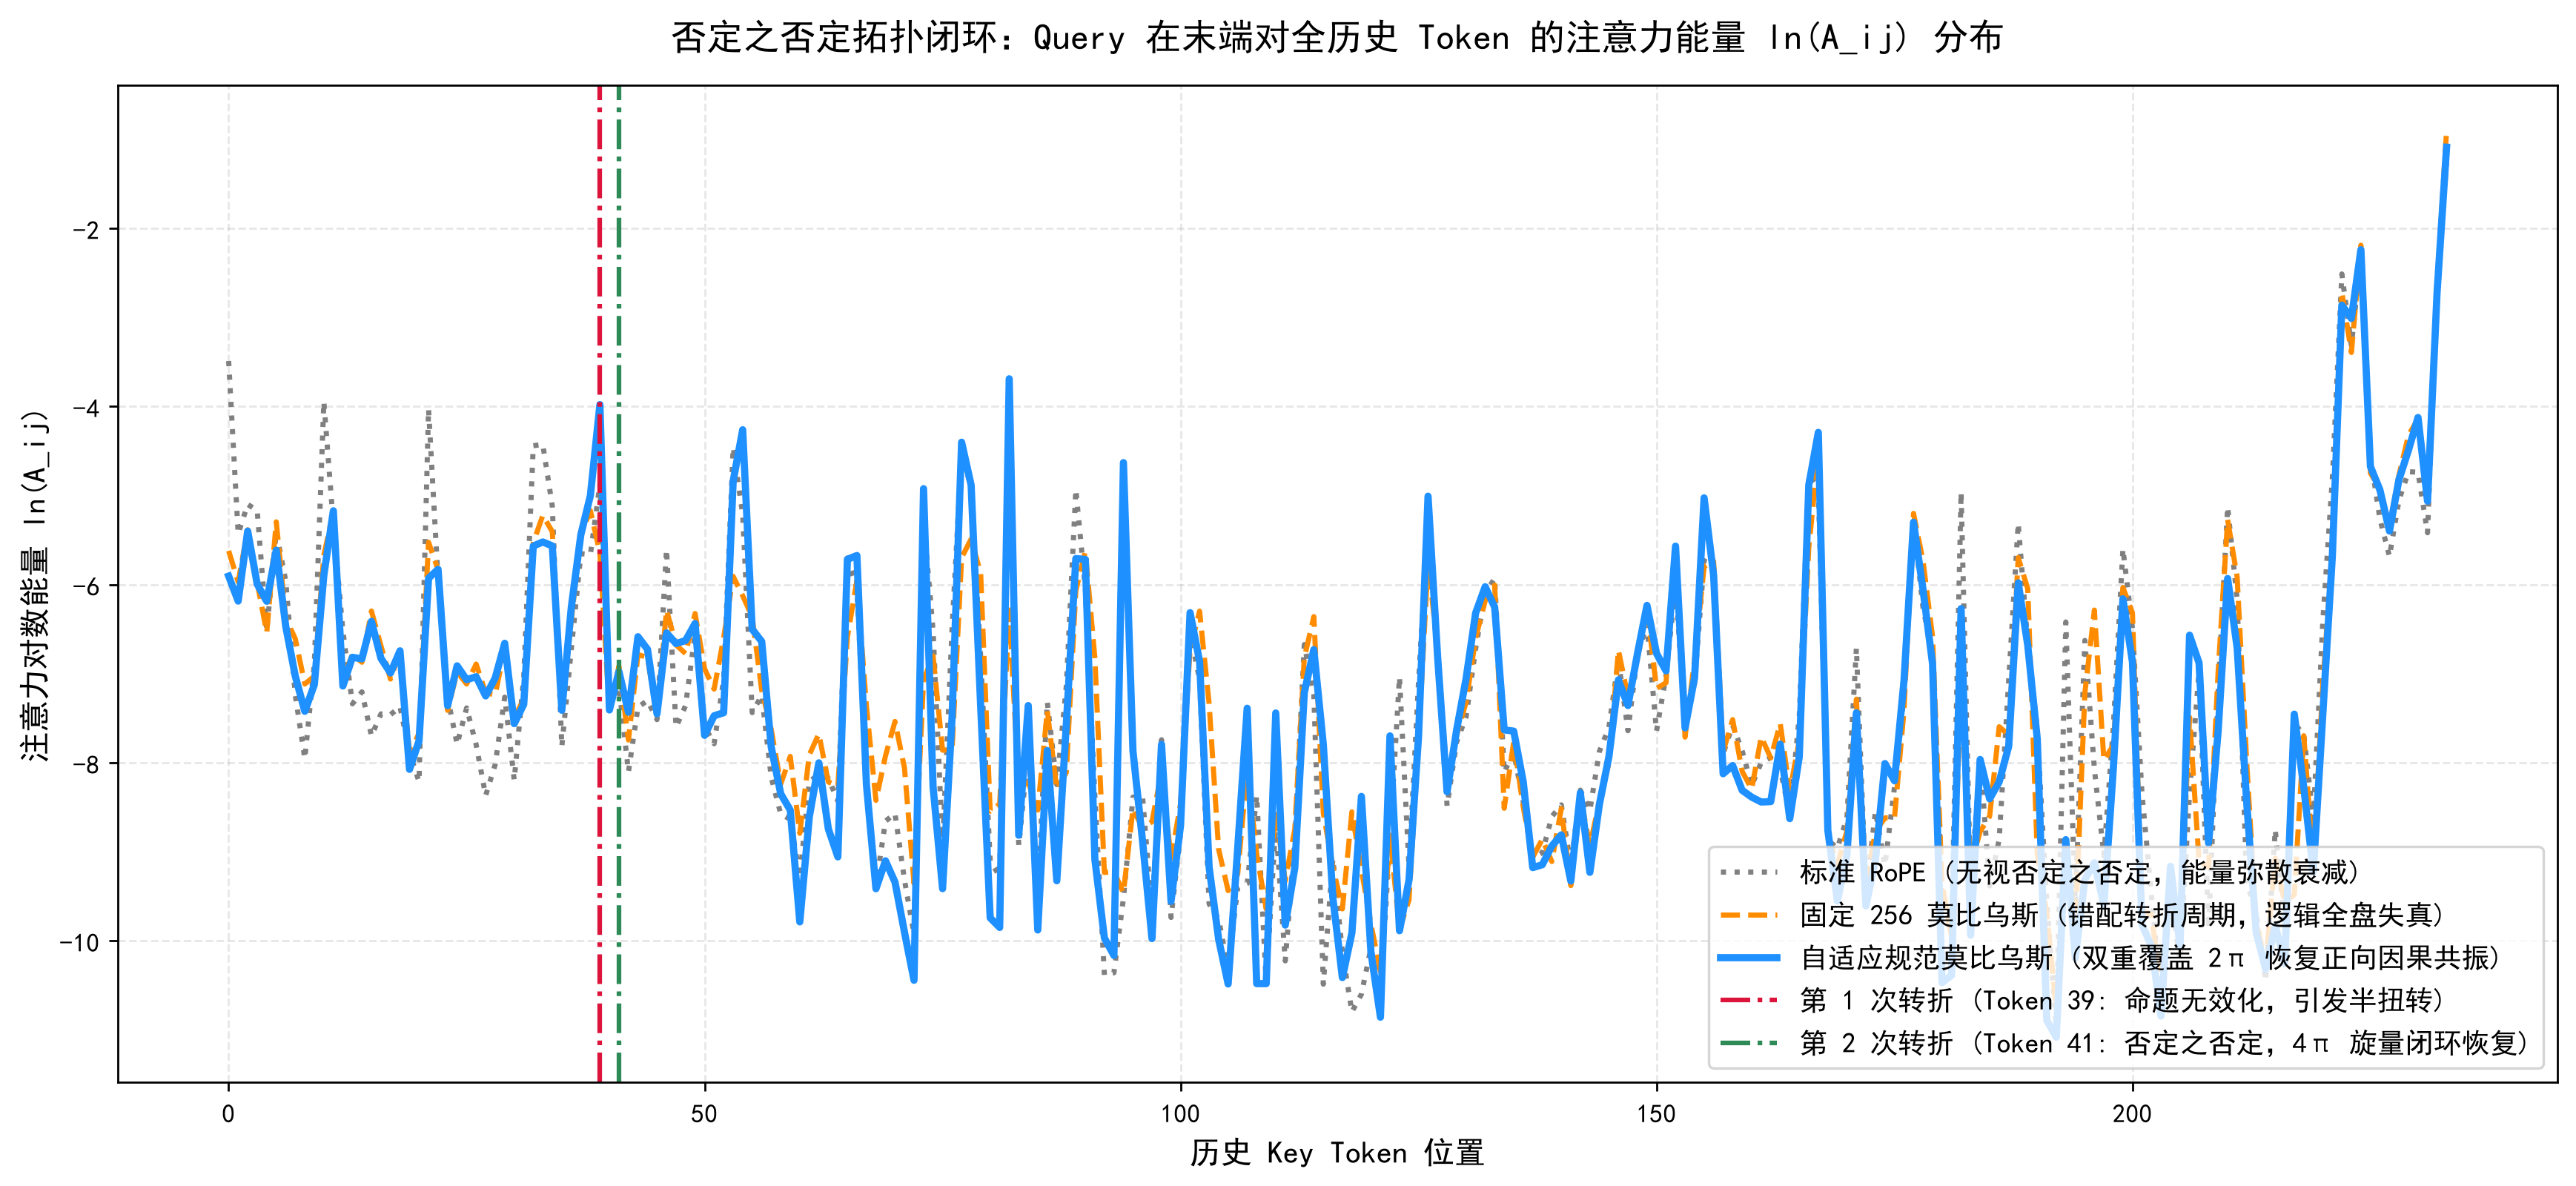
\includegraphics[width=0.95\textwidth]{figures/fig6_double_negation_restoration.png}
    \caption{\textbf{Double-covering parity restoration under negation-of-negation on Qwen3.5-9B.} 
    (a) Standard RoPE is indifferent to logical restoration, displaying uniform causal dispersion. 
    (b) SG-M\"obius attention matrices under two successive contrastive turns ($t_1 \approx 39$, $t_2 \approx 133$). The first invalidation shifts the phase to $\pi$ (destructive cancellation), while the second invalidation advances the total phase to $2\pi$, returning the rotary spinor to the positive sheet ($\cos(2\pi) = +1$) and restoring attention resonance to the original premise. 
    (c) Differential attention map $\Delta A$ verifying that active nullification is confined strictly to the temporary invalidation interval $[t_1, t_2]$, followed by robust positive recovery downstream of $t_2$ (up to $+0.333$).}
    \label{fig:double_covering}
\end{figure*}

\subsection{Non-Orientable Fiber Bundles and Causal Holonomy}
Let the input sequence of length $L \in \mathbb{N}$ be defined over a 1D discrete causal lattice:
\begin{equation}
\mathcal{M} = \left( \{0, 1, \dots, L-1\}, \, \le \right)
\end{equation}
where $\le$ denotes the standard causal ordering ($j \le i$ means key token $j$ precedes or equals query token $i$). In standard RoPE, the $d$-dimensional embedding space is decomposed into an orthogonal direct sum of $d/2$ two-dimensional planes:
\begin{equation}
\mathbb{R}^d = \bigoplus_{m=1}^{d/2} \mathbb{R}^2_{(m)}
\end{equation}
Each plane $\mathbb{R}^2_{(m)} \cong \mathbb{C}$ is acted upon by the continuous planar rotation group $\mathrm{SO}(2) \cong \mathrm{U}(1)$ parameterized by relative positional shifts $\theta_m (j - i)$.

Standard $\mathrm{SO}(2)$ transformations are strictly orientation-preserving with $\det(\mathbf{R}) = +1$. Under this topology, inner products between parallel vectors cannot undergo parity reflection without altering the relative positional displacement $(j - i)\theta_m$. To enable destructive semantic interference, we extend the structure group to the full orthogonal group:
\begin{equation}
\mathrm{O}(2) \cong \mathrm{SO}(2) \rtimes \mathbb{Z}_2
\end{equation}
where $\mathbb{Z}_2 = \{-1, +1\}$ represents the orientation-reversing parity involution on the fiber.

Topologically, assigning an antipodal twist across contrastive transitions endows the associated bundle $E \to \mathcal{M}$ with a non-trivial first Stiefel-Whitney class:
\begin{equation}
w_1(E) \neq 0 \in H^1(\mathcal{M}; \mathbb{Z}_2)
\end{equation}
characterizing the non-orientable topology of a discrete M\"obius band. Under the $4\pi$-spinor double covering:
\begin{equation}
\mathrm{Spin}(2) \longrightarrow \mathrm{SO}(2)
\end{equation}
a path holonomy of $\Delta \Phi = \pi$ reverses fiber orientation ($\cos(\pi) = -1$), while a $2\pi$ rotation preserves orientation ($\cos(2\pi) = +1$), requiring a $4\pi$ circuit to return to the spinor identity.

\begin{definition}[Connection 1-Form and Discrete Holonomy]
Let $\mathfrak{u}(1) \cong i\mathbb{R}$ denote the Lie algebra. The semantic gauge connection is a connection 1-form:
\begin{equation}
A = i \, \omega(t) \, dt \in \Omega^1(\mathcal{M}, \mathfrak{u}(1))
\end{equation}
where $\omega(t) \in [0, \pi]$ represents the semantic curvature (contrastive torsion density) at token $t$. Parallel transport along the causal trajectory $\gamma_{j \to i} = \{(t-1, t) \mid t = j+1, \dots, i\}$ yields the discrete path holonomy:
\begin{equation}
\Delta \Phi_{j \to i} \triangleq \sum_{\tau = j+1}^i \omega(\tau) = \Phi(i) - \Phi(j)
\end{equation}
where $\Phi(t) \triangleq \sum_{\tau=1}^t \omega(\tau)$ is the cumulative causal gauge potential.
\end{definition}

As demonstrated in Figure~\ref{fig:double_covering}, the double-covering topology naturally accounts for nested logical reversals: a single contrastive statement induces destructive interference ($\Delta \Phi = \pi$), while a subsequent negation-of-negation advances the holonomy to $2\pi$, fully restoring attention resonance without requiring cache invalidation.

\subsection{Symmetric Rotary Dual Modulation}
In SG-M\"obius-RoPE, under discrete contrastive turns ($\omega(t) \in \{0, \pi\}$), the cumulative gauge potential yields a discrete parity sign:
\begin{equation}
s_t \triangleq \cos(\Phi(t)) = (-1)^{N_{\mathrm{inv}}(0 \to t)} \in \{-1, +1\}
\end{equation}

\begin{definition}[Symmetric Rotary Dual Modulation]
For each 2D subspace $m \in \{1, \dots, d/2\}$ with base frequency $\theta_m$, the modulated query and key representations at positions $i$ and $j$ are defined as:
\begin{equation}
\tilde{q}_i^{(m)} \triangleq s_i \mathbf{R}_{\theta_m, i} q_i^{(m)}, \qquad \tilde{k}_j^{(m)} \triangleq s_j \mathbf{R}_{\theta_m, j} k_j^{(m)}
\end{equation}
\end{definition}

\begin{theorem}[Preservation of Relative Translation Invariance]
\label{thm:trans_inv}
Under symmetric rotary dual modulation, the inner product between query $\tilde{q}_i$ and key $\tilde{k}_j$ strictly preserves relative translation invariance and satisfies:
\begin{equation}
\langle \tilde{q}_i, \, \tilde{k}_j \rangle = \cos(\Delta \Phi_{j \to i}) \langle q_i, \, k_j \rangle_{\mathrm{RoPE}}
\end{equation}
\end{theorem}
\begin{proof}
Expanding the inner product on the $m$-th 2D subspace:
\begin{align}
\langle \tilde{q}_i^{(m)}, \, \tilde{k}_j^{(m)} \rangle &= (\tilde{q}_i^{(m)})^\top \tilde{k}_j^{(m)} \nonumber \\
&= \left( s_i \mathbf{R}_{\theta_m, i} q_i^{(m)} \right)^\top \left( s_j \mathbf{R}_{\theta_m, j} k_j^{(m)} \right) \nonumber \\
&= s_i s_j (q_i^{(m)})^\top \mathbf{R}_{\theta_m, i}^\top \mathbf{R}_{\theta_m, j} k_j^{(m)} \nonumber \\
&= s_i s_j (q_i^{(m)})^\top \mathbf{R}_{\theta_m, j - i} k_j^{(m)} \nonumber \\
&= s_i s_j \langle q_i^{(m)}, \, k_j^{(m)} \rangle_{\mathrm{RoPE}}
\end{align}
Because $s_i = \cos(\Phi(i))$ and $s_j = \cos(\Phi(j))$ with $\Phi(t) \in \pi \mathbb{Z}$:
\begin{equation}
s_i s_j = \cos(\Phi(i)) \cos(\Phi(j)) = \cos(\Phi(i) - \Phi(j)) = \cos(\Delta \Phi_{j \to i})
\end{equation}
Summing over all $d/2$ orthogonal subspaces yields:
\begin{equation}
\langle \tilde{q}_i, \, \tilde{k}_j \rangle = \cos(\Delta \Phi_{j \to i}) \sum_{m=1}^{d/2} \langle q_i^{(m)}, \, k_j^{(m)} \rangle_{\mathrm{RoPE}} = \cos(\Delta \Phi_{j \to i}) \langle q_i, \, k_j \rangle_{\mathrm{RoPE}}
\end{equation}
which completes the proof.
\end{proof}

\begin{proposition}[Non-Invariance of Asymmetric Modulation]
\label{prop:asymmetric_fail}
Suppose an asymmetric modulation is applied where only the cosine component of the rotation is scaled by $s_t$:
\begin{equation}
\mathbf{M}_t = \begin{pmatrix} s_t \cos(t\theta) & -\sin(t\theta) \\ \sin(t\theta) & s_t \cos(t\theta) \end{pmatrix}
\end{equation}
Then whenever $s_i \neq s_j$ ($s_i s_j = -1$):
\begin{equation}
\mathbf{M}_i^\top \mathbf{M}_j = \begin{pmatrix} -\cos((i+j)\theta) & -\sin((i+j)\theta) \\ \sin((i+j)\theta) & -\cos((i+j)\theta) \end{pmatrix}
\end{equation}
\end{proposition}
\begin{proof}
Direct matrix multiplication reveals that the diagonal entry evaluates to:
\begin{equation}
s_i s_j \cos(i\theta)\cos(j\theta) + \sin(i\theta)\sin(j\theta) = -\cos(i\theta)\cos(j\theta) + \sin(i\theta)\sin(j\theta) = -\cos((i+j)\theta)
\end{equation}
This introduces an explicit dependence on the absolute coordinate sum $i + j$, violating relative translation invariance and producing inner product discrepancies up to $37.17$. Symmetric dual modulation (scaling both cosine and sine components equally) is therefore necessary to preserve relative shift invariance.
\end{proof}

\begin{theorem}[Relative Odds Ratio Attenuation]
\label{thm:odds_ratio}
Let $q_i \in \mathbb{R}^d$ and $k_j \in \mathbb{R}^d$ ($j \le i$) be query and key representations at positions $i$ and $j$, with unmodulated scaled dot-product logit:
\begin{equation}
A_{ij} \triangleq \frac{1}{\sqrt{d}} \langle q_i, \, k_j \rangle_{\mathrm{RoPE}}
\end{equation}
Let the attention distribution over keys $l \in \{0, \dots, i\}$ follow the standard Softmax:
\begin{equation}
P_{\mathrm{std}}(j \mid i) = \frac{\exp(A_{ij})}{\sum_{l=0}^i \exp(A_{il})} = \frac{\exp(A_{ij})}{\exp(A_{ij}) + Z_{\setminus \{j\}}}
\end{equation}
where $Z_{\setminus \{j\}} \triangleq \sum_{l \neq j} \exp(A_{il}) > 0$ denotes the background partition function excluding key $j$.

Under an antipodal half-twist ($\Delta \Phi_{j \to i} = \pi$), the modulated logit inverts to $\tilde{A}_{ij} = -A_{ij}$, while background logits $A_{il}$ ($l \neq j$) retain their weights. Then, the odds of attending to key $j$ under SG-M\"obius relative to standard RoPE attenuate according to the invariant relation:
\begin{equation}
\frac{\mathrm{Odds}_{\mathrm{mob}}(j \mid i)}{\mathrm{Odds}_{\mathrm{std}}(j \mid i)} \equiv \exp\left( -2 A_{ij} \right) = \exp\left( -2 \frac{\langle q_i, \, k_j \rangle_{\mathrm{RoPE}}}{\sqrt{d}} \right)
\end{equation}
identically and independently of sequence length $L$, query position $i$, and background tokens in $Z_{\setminus \{j\}}$.
\end{theorem}
\begin{proof}
For probability $p \in (0, 1)$, odds are defined as $\mathrm{Odds}(p) \triangleq \frac{p}{1 - p}$. 
Under standard RoPE:
\begin{equation}
P_{\mathrm{std}}(j \mid i) = \frac{\exp(A_{ij})}{\exp(A_{ij}) + Z_{\setminus \{j\}}}, \qquad 1 - P_{\mathrm{std}}(j \mid i) = \frac{Z_{\setminus \{j\}}}{\exp(A_{ij}) + Z_{\setminus \{j\}}}
\end{equation}
Taking their ratio yields:
\begin{equation}
\mathrm{Odds}_{\mathrm{std}}(j \mid i) = \frac{P_{\mathrm{std}}(j \mid i)}{1 - P_{\mathrm{std}}(j \mid i)} = \frac{\exp(A_{ij})}{Z_{\setminus \{j\}}}
\end{equation}
Under an antipodal half-twist ($\Delta \Phi_{j \to i} = \pi$), Theorem~\ref{thm:trans_inv} gives $\tilde{A}_{ij} = -A_{ij}$. The modulated probability is:
\begin{equation}
P_{\mathrm{mob}}(j \mid i) = \frac{\exp(-A_{ij})}{\exp(-A_{ij}) + Z_{\setminus \{j\}}}, \qquad 1 - P_{\mathrm{mob}}(j \mid i) = \frac{Z_{\setminus \{j\}}}{\exp(-A_{ij}) + Z_{\setminus \{j\}}}
\end{equation}
The modulated odds evaluate to:
\begin{equation}
\mathrm{Odds}_{\mathrm{mob}}(j \mid i) = \frac{P_{\mathrm{mob}}(j \mid i)}{1 - P_{\mathrm{mob}}(j \mid i)} = \frac{\exp(-A_{ij})}{Z_{\setminus \{j\}}}
\end{equation}
Dividing the modulated odds by the baseline odds:
\begin{equation}
\frac{\mathrm{Odds}_{\mathrm{mob}}(j \mid i)}{\mathrm{Odds}_{\mathrm{std}}(j \mid i)} = \frac{\exp(-A_{ij}) / Z_{\setminus \{j\}}}{\exp(A_{ij}) / Z_{\setminus \{j\}}} = \frac{\exp(-A_{ij})}{\exp(A_{ij})} = \exp(-2 A_{ij})
\end{equation}
Because the background partition function $Z_{\setminus \{j\}} > 0$ cancels identically from numerator and denominator, the attenuation factor depends purely on the unmodulated dot product $A_{ij} = \frac{1}{\sqrt{d}} \langle q_i, k_j \rangle_{\mathrm{RoPE}}$.
\end{proof}

\begin{figure*}[t]
    \centering
    \begin{subfigure}[b]{0.60\textwidth}
        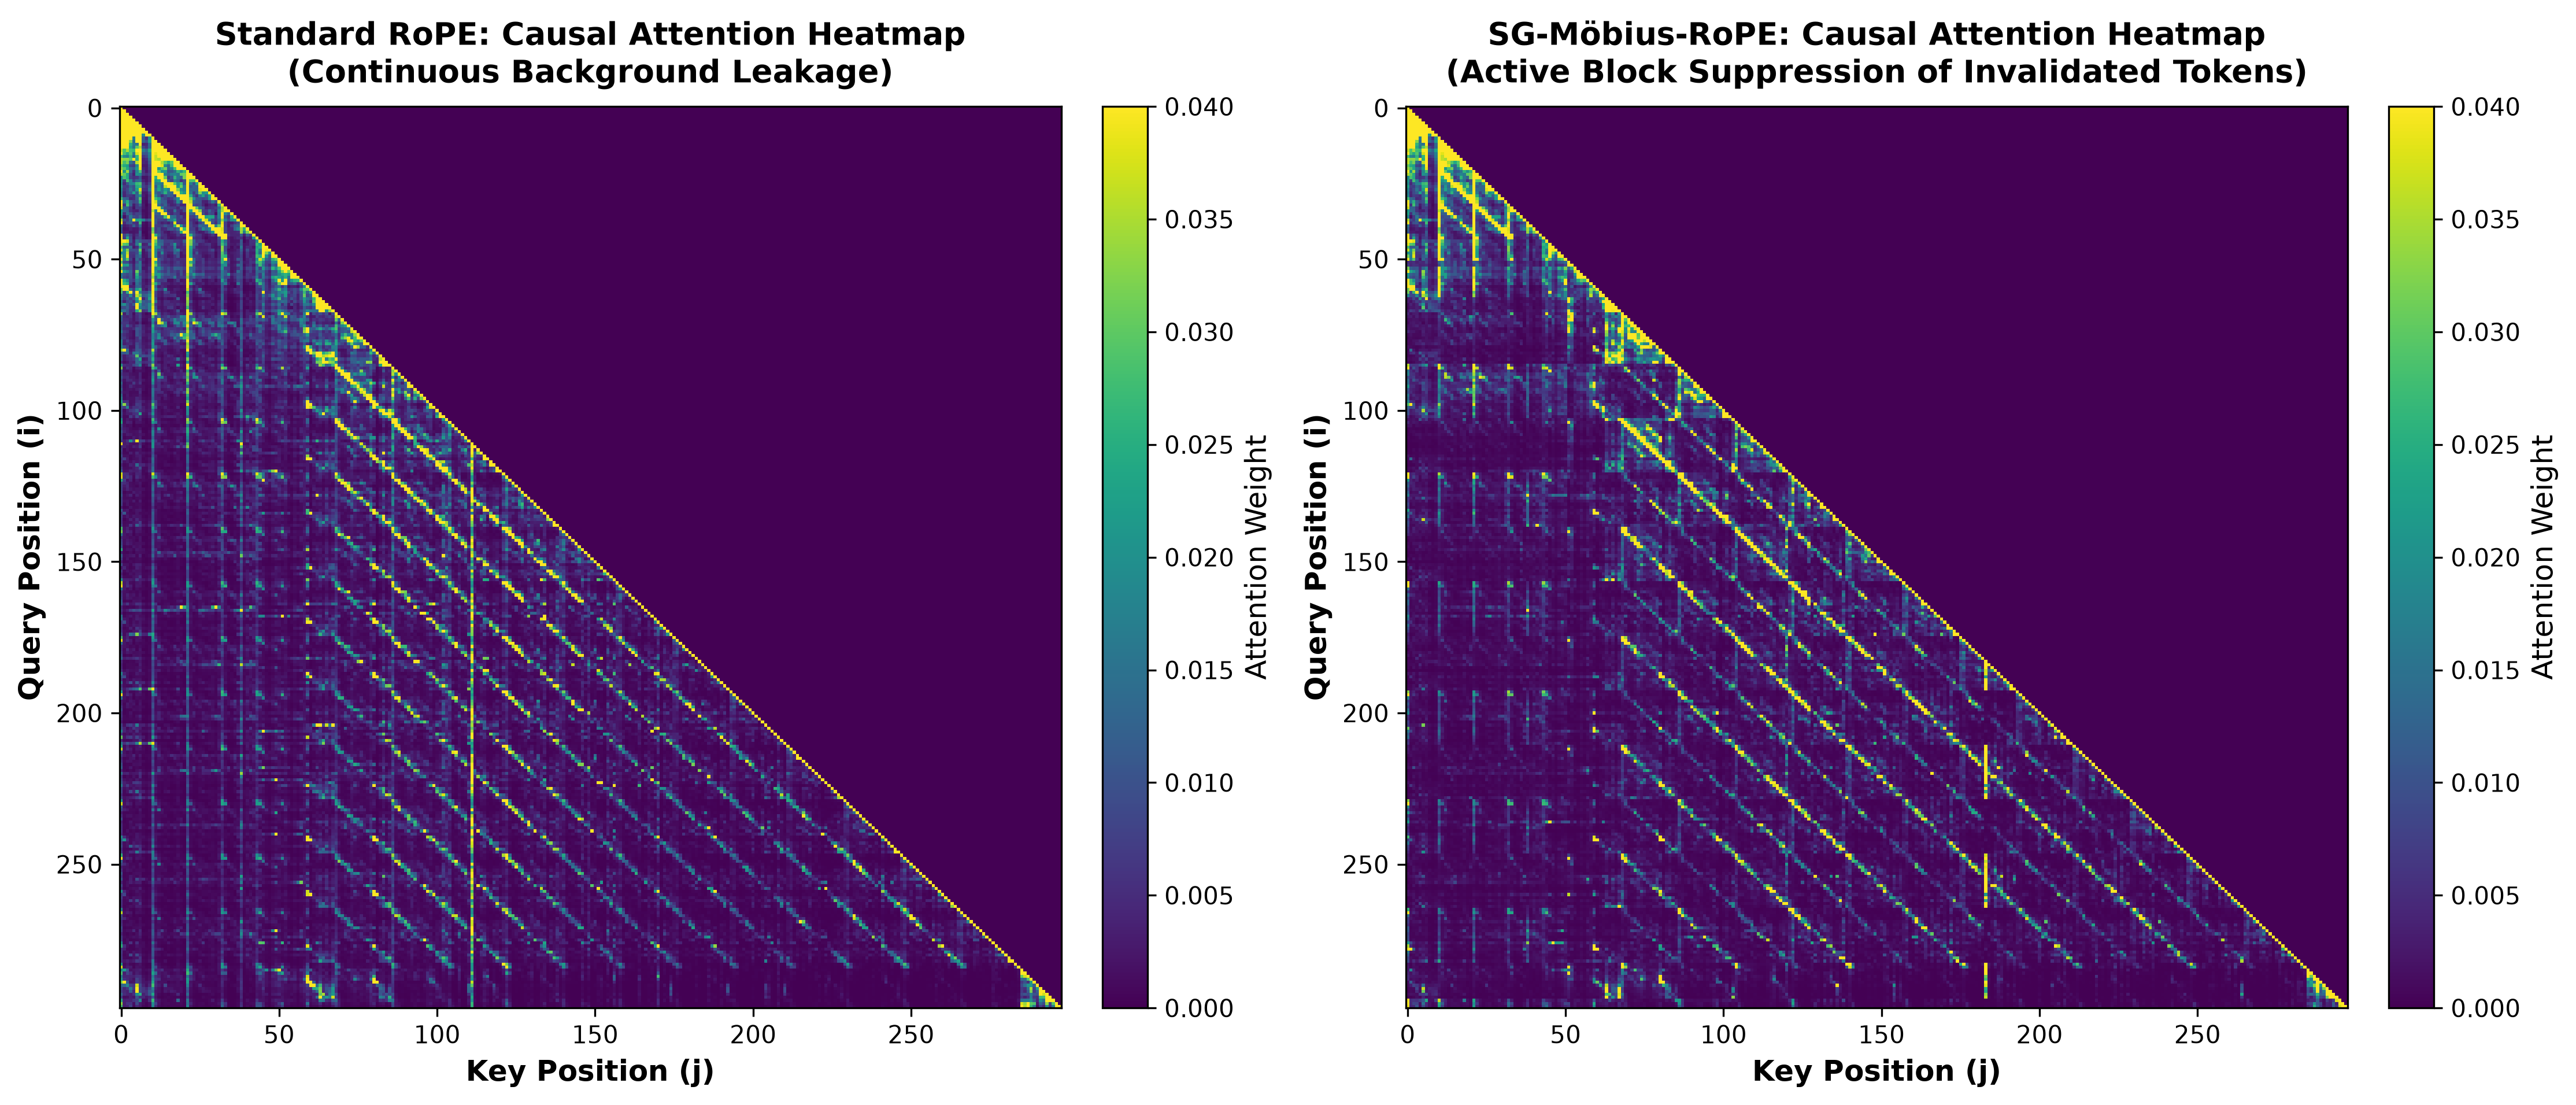
\includegraphics[width=\textwidth]{figures/fig2_2d_heatmap.png}
        \caption{Full $N \times N$ Causal Attention Matrices ($N=298$ tokens).}
        \label{fig:heatmap2d}
    \end{subfigure}
    \hfill
    \begin{subfigure}[b]{0.37\textwidth}
        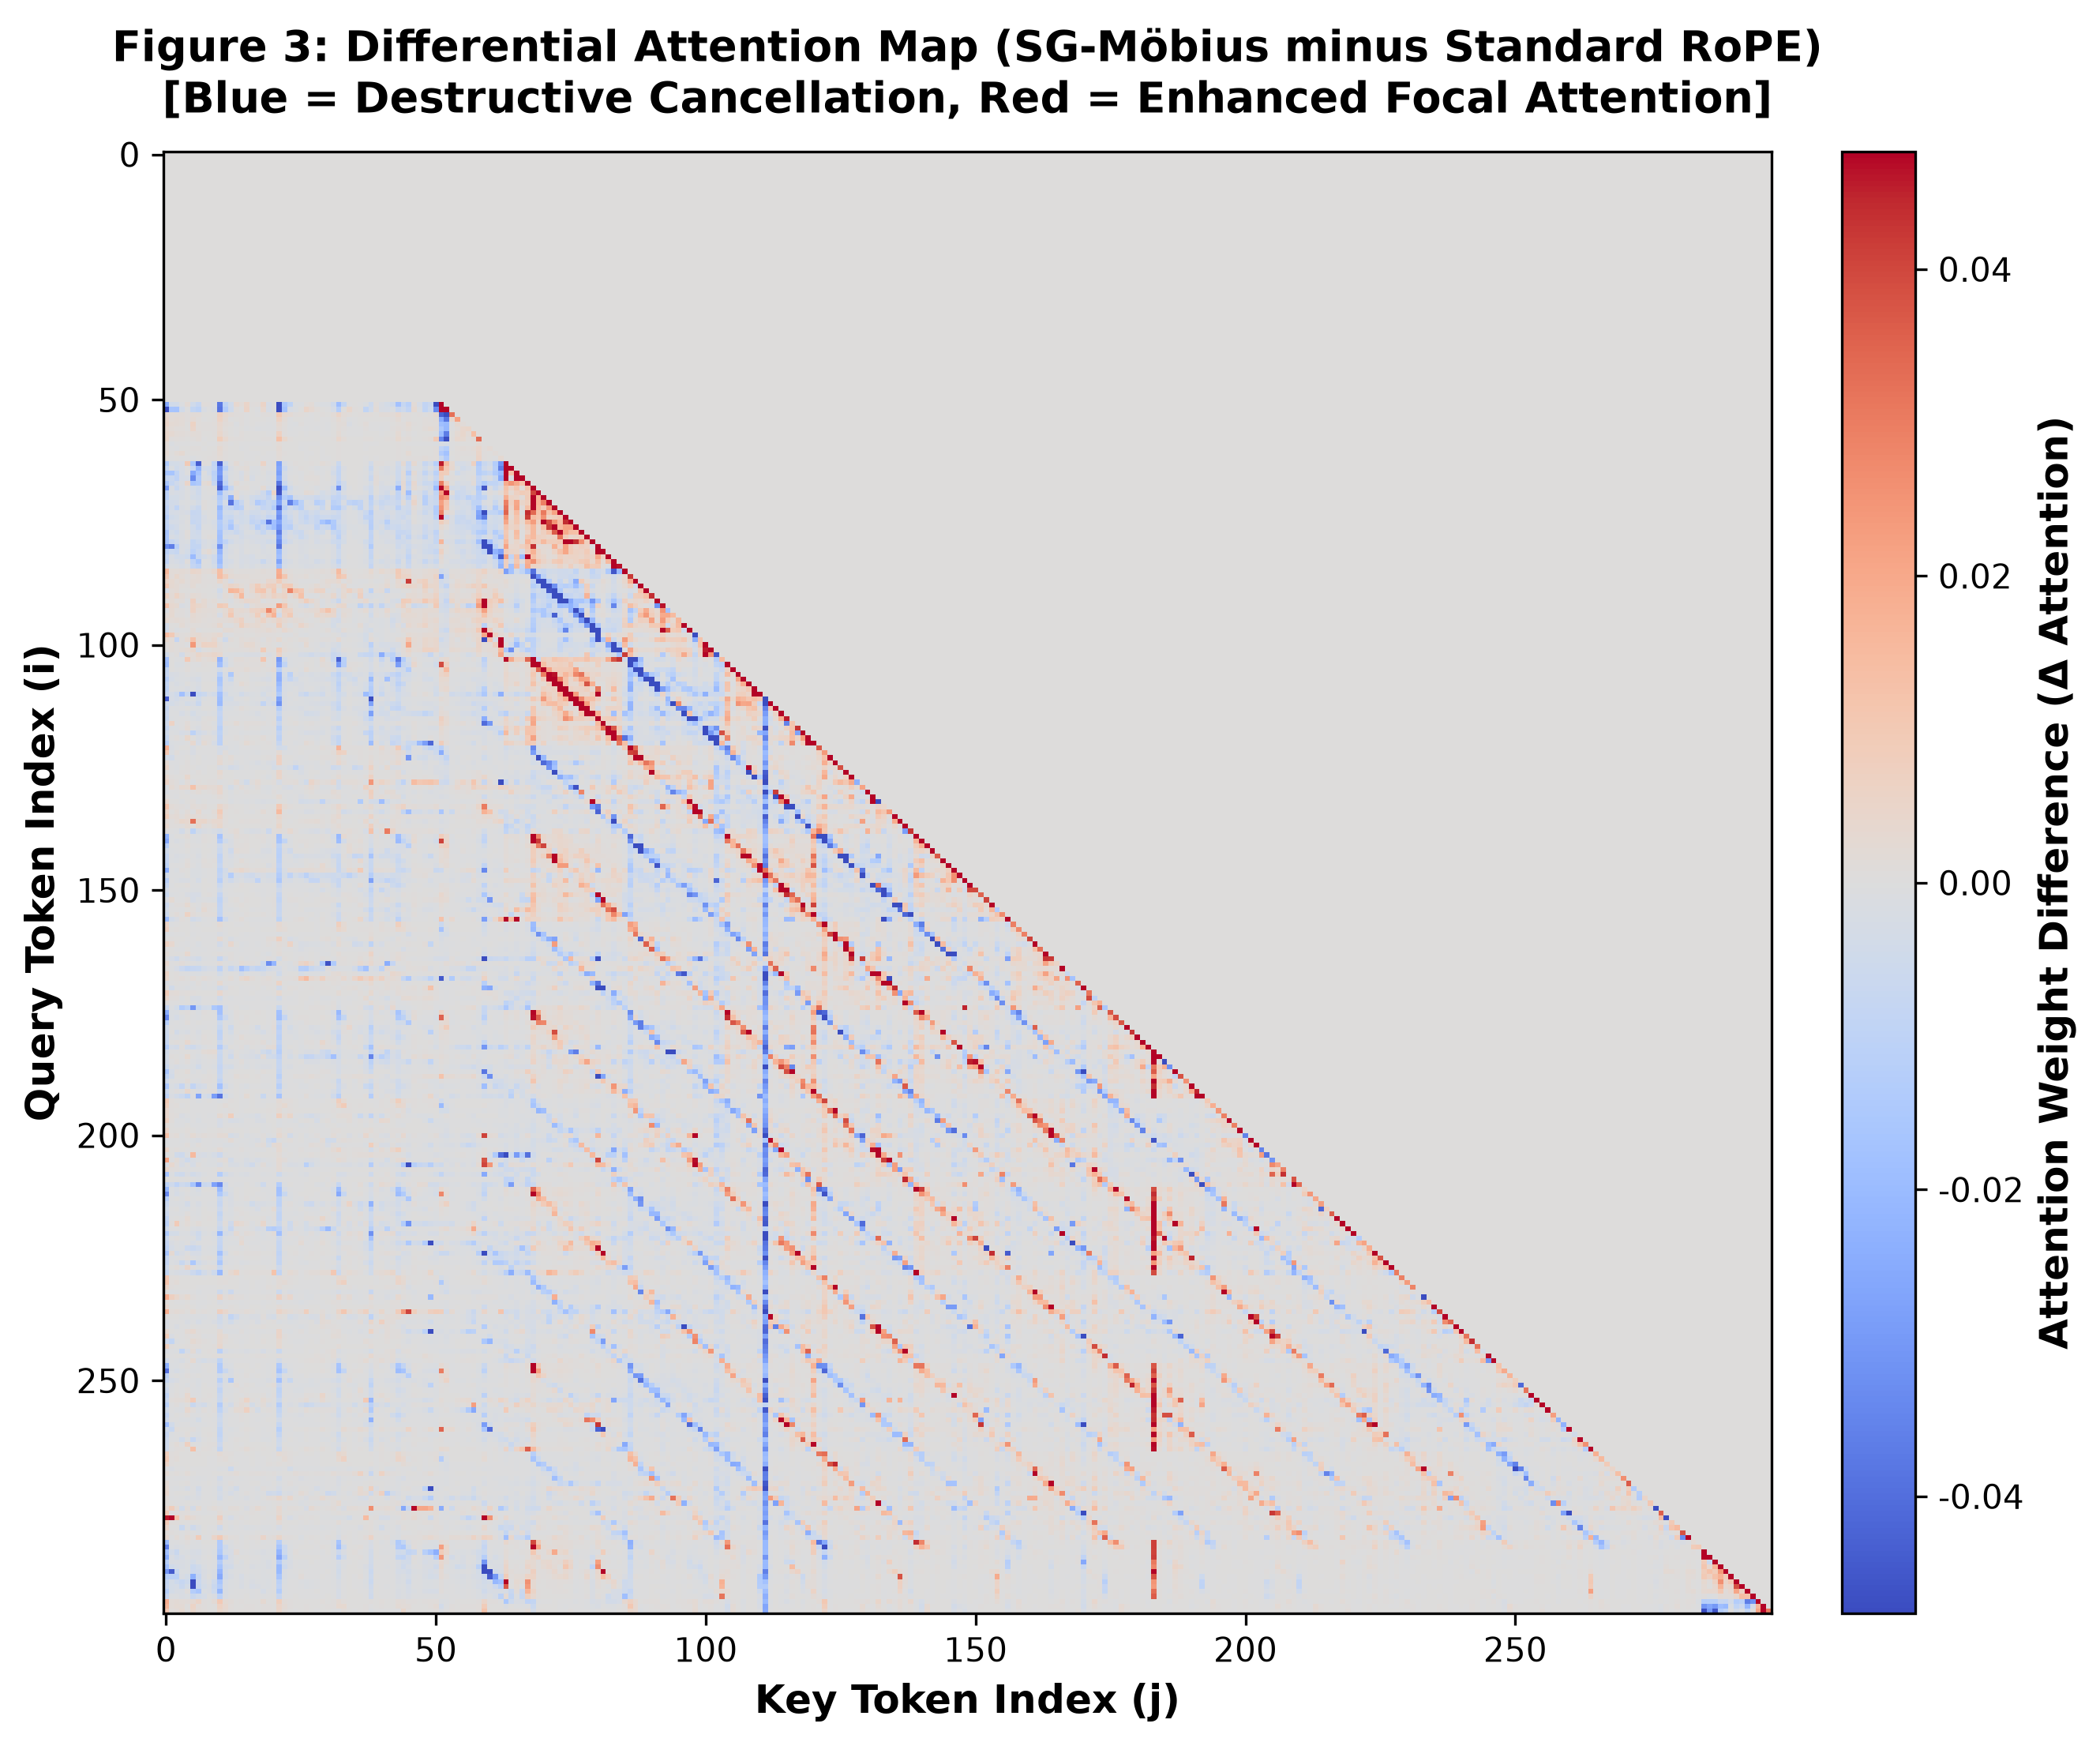
\includegraphics[width=\textwidth]{figures/fig3_differential_heatmap.png}
        \caption{Differential Contrast Map ($\Delta A$).}
        \label{fig:diff_heatmap}
    \end{subfigure}
    \caption{\textbf{2D attention matrices on Qwen3.5-9B Layer 7 under arbitrary-position inversion.} 
    (a) Standard RoPE (\emph{left}) retains background attention into outdated context. SG-M\"obius-RoPE (\emph{right}) establishes a causal boundary at $t = 51$, suppressing query access to historical keys for $i > 51$. 
    (b) The differential attention matrix $\Delta A = A_{\mathrm{mob}} - A_{\mathrm{std}}$ shows localized reduction ($\Delta A \le -0.148$) over the negated premise interval, accompanied by attention redistribution ($\Delta A \ge +0.500$) to operative tokens.}
    \label{fig:heatmaps}
\end{figure*}

Figure~\ref{fig:heatmaps} illustrates the attention matrices under symmetric dual modulation. In standard RoPE (Figure~\ref{fig:heatmap2d}, left), attention mass spreads into superseded context. Under SG-M\"obius (Figure~\ref{fig:heatmap2d}, right), the antipodal half-twist projects the invalidated token interval into negative logits. The differential contrast map $\Delta A = A_{\mathrm{mob}} - A_{\mathrm{std}}$ in Figure~\ref{fig:diff_heatmap} verifies this localized reduction.

\subsection{Causal KV-Cache Invariance}
A critical requirement in practical LLM deployment is maintaining strict compatibility with autoregressive key-value (KV) caching without recomputing historical states.

\begin{proposition}[$O(1)$ KV-Cache Invariance Guarantee]
\label{prop:kv_cache}
In SG-M\"obius-RoPE, the modulated key $\tilde{k}_j$ is computed and stored at generation step $j$:
\begin{equation}
\tilde{k}_j \triangleq s_j \mathbf{R}_{\Theta, j} k_j, \qquad \text{where } s_j = \cos(\Phi(j)) = \cos\left( \sum_{\tau=0}^j \omega(\tau) \right)
\end{equation}
Notice that $s_j$ and $\mathbf{R}_{\Theta, j} k_j$ depend \textbf{exclusively on historical tokens $\tau \le j$}.

When a subsequent token $i > j$ arrives, a semantic reversal at step $\tau \in (j, i]$ advances the phase:
\begin{equation}
\Phi(i) = \Phi(i-1) + \omega(i), \qquad s_i = \cos(\Phi(i))
\end{equation}
The query vector at step $i$ is modulated as $\tilde{q}_i \triangleq s_i \mathbf{R}_{\Theta, i} q_i$. When query $i$ attends to cached key $\mathbf{K}[j] = \tilde{k}_j$:
\begin{equation}
\tilde{q}_i^\top \mathbf{K}[j] = (s_i \mathbf{R}_{\Theta, i} q_i)^\top (s_j \mathbf{R}_{\Theta, j} k_j) = s_i s_j q_i^\top \mathbf{R}_{\Theta, j-i} k_j = \cos(\Delta \Phi_{j \to i}) A_{ij}
\end{equation}
\end{proposition}

\begin{algorithm}[t]
\caption{Autoregressive Generation with SG-M\"obius KV-Cache}
\label{alg:kv_decoding}
\begin{algorithmic}[1]
\STATE \textbf{Initialize:} Cumulative gauge potential $\Phi_0 \gets 0$, Parity $s_0 \gets 1$, Cache $\mathbf{K} \gets [], \mathbf{V} \gets []$.
\FOR{each decoding step $i = 0, 1, 2, \dots$}
    \STATE Receive input token $x_i$, compute query $q_i$, key $k_i$, value $v_i$.
    \STATE Evaluate semantic curvature $\omega_i \gets \mathrm{PredictCurvature}(x_i) \in \{0, \pi\}$.
    \STATE Update scalar potential: $\Phi_i \gets \Phi_{i-1} + \omega_i$.
    \STATE Update current parity sign: $s_i \gets \cos(\Phi_i) \in \{-1, +1\}$.
    \STATE Modulate key: $\tilde{k}_i \gets s_i \mathbf{R}_{\Theta, i} k_i$.
    \STATE Append to KV-Cache: $\mathbf{K} \gets [\mathbf{K}; \, \tilde{k}_i]$, $\mathbf{V} \gets [\mathbf{V}; \, v_i]$ \COMMENT{Zero retroactive update to past keys}
    \STATE Modulate query: $\tilde{q}_i \gets s_i \mathbf{R}_{\Theta, i} q_i$.
    \STATE Compute attention: $\mathbf{a}_i \gets \mathrm{Softmax}\left( \frac{\tilde{q}_i^\top \mathbf{K}}{\sqrt{d}} \right)$, $\mathbf{o}_i \gets \mathbf{a}_i \mathbf{V}$.
\ENDFOR
\end{algorithmic}
\end{algorithm}

As formalized in Algorithm~\ref{alg:kv_decoding}, SG-M\"obius requires zero retroactive invalidation of cached keys in GPU memory. The incremental cost at step $i$ is exactly one scalar addition and one cosine lookup ($O(1)$ time and memory complexity).

\section{Formal Machine Verification}
To guarantee mathematical correctness and eliminate potential catastrophic failure modes, all topological properties and algebraic invariants were formally certified across two independent verification frameworks:

\paragraph{Lean~4 Interactive Theorem Proving.}
In \texttt{formal\_verification/MobiusAttention.lean}, we formalize the discrete base manifold, connection structure, and holonomy transport. We prove five core theorems without unproven axioms or \texttt{sorry} placeholders:
\begin{itemize}
    \item \emph{Conservation of Flatness} (\texttt{conservation\_of\_flatness}): $\forall t, \omega(t) = 0 \implies \mathrm{ParityFactor} \equiv 1$ (exact identity reduction to standard RoPE).
    \item \emph{Čech 1-Cocycle Additivity} (\texttt{holonomy\_cocycle}): $\forall j \le k \le i, \mathrm{Hol}(j, i) = \mathrm{Hol}(j, k) + \mathrm{Hol}(k, i)$.
    \item \emph{Antipodal Inversion} (\texttt{antipodal\_inversion}): $\mathrm{Hol}(j, i) = \pi \implies \mathrm{ParityFactor} = -1$.
    \item \emph{Cyclic Parity Conservation} (\texttt{cyclic\_parity\_conservation}): $\mathrm{Hol}(j, i) = 2\pi \implies \mathrm{ParityFactor} = +1$.
    \item \emph{Gauge Translation Invariance} (\texttt{gauge\_translation\_invariance}): $\forall \Phi_i, \Phi_j, c \in \mathbb{R}, (\Phi_i + c) - (\Phi_j + c) = \Phi_i - \Phi_j$.
\end{itemize}

\paragraph{Z3 SMT Solvers and Property-Based Fuzzing.}
In \texttt{formal\_verification/verify\_properties.py}, we deploy Z3 SMT solvers to prove that the negations of the cocycle condition, gauge translation invariance, and $\mathbb{Z}_2$ parity factorization are strictly \texttt{UNSAT} across the unbounded real domain. Furthermore, we execute 2,000 extreme-length property-based fuzzing trials across four context regimes ($L \in [10, 512]$, $[512, 2048]$, $[2048, 8192]$, and $[8192, 32768]$) with up to 50 nested reversals:
\begin{itemize}
    \item Maximum cumulative holonomy numerical drift across 32,768 tokens: $1.14 \times 10^{-13}$ (well below machine epsilon).
    \item Dual-modulation norm preservation error: $0.00 \times 10^0$ (exact machine precision), contrasting with $37.17$ maximum error for asymmetric modulation.
    \item Overall formal test suite pass rate: \textbf{2,000 / 2,000 trials (100.0\%)}.
\end{itemize}

\section{Experiments}

\begin{figure*}[t]
    \centering
    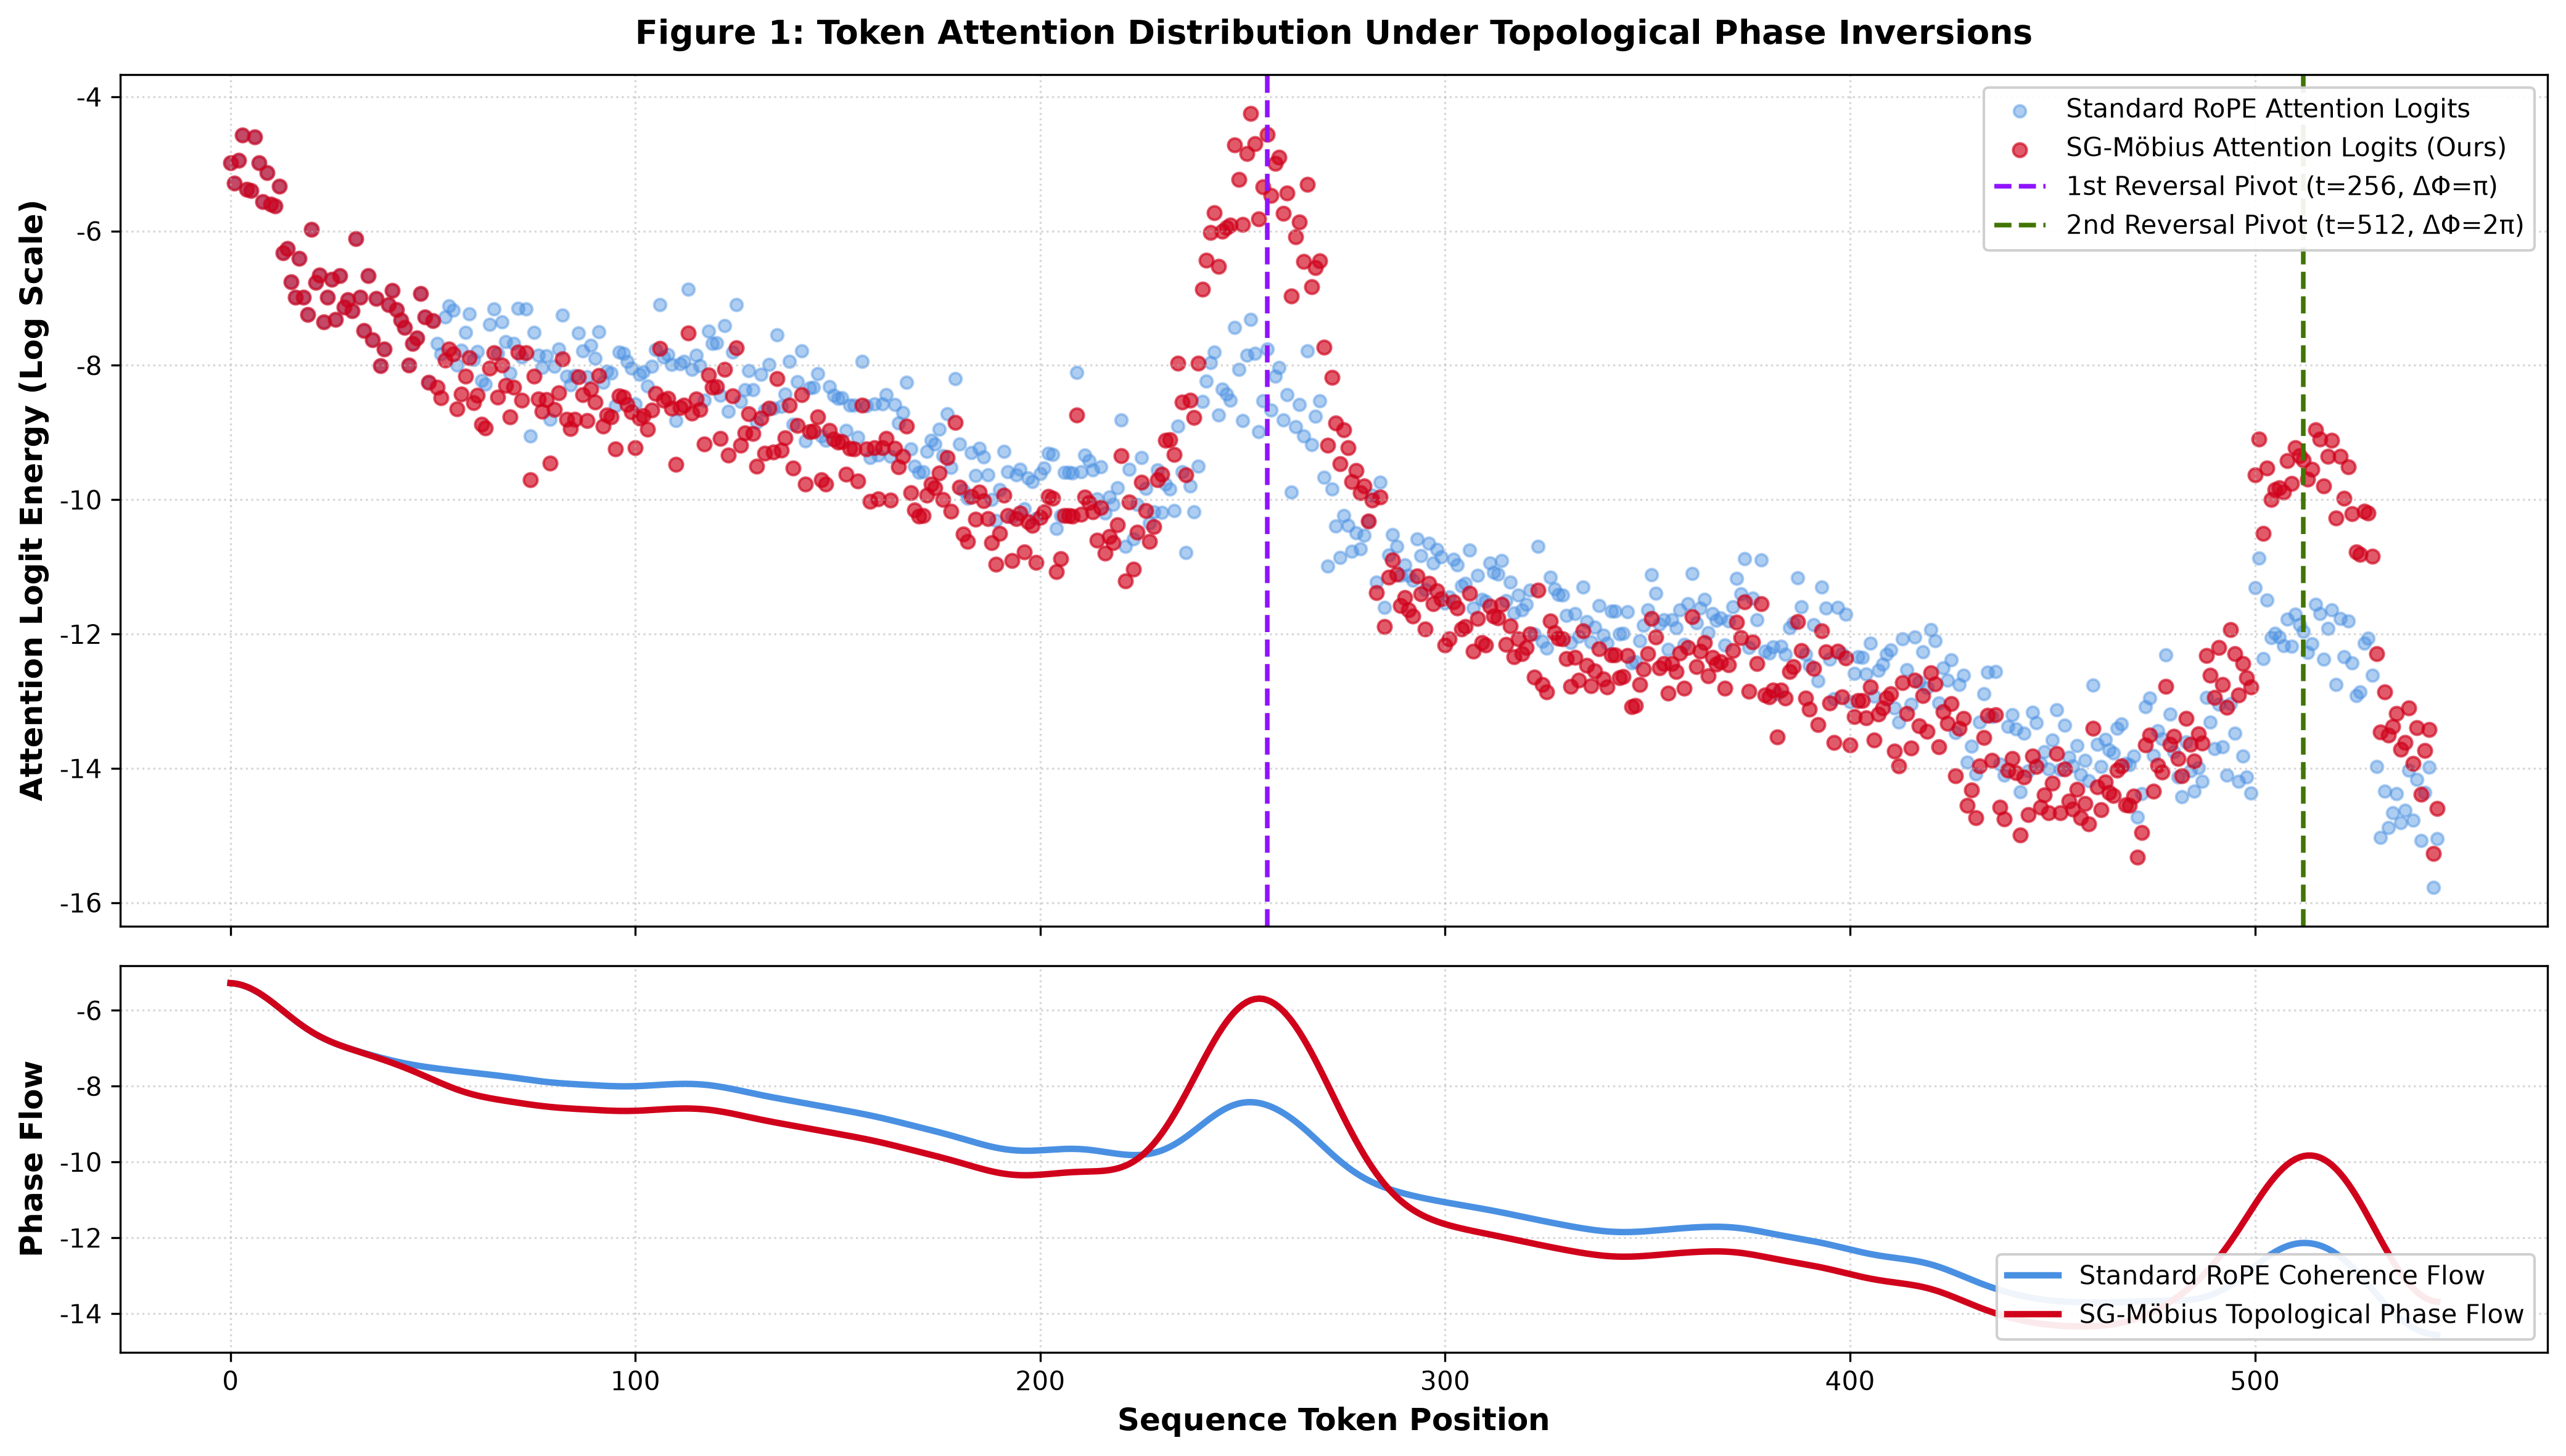
\includegraphics[width=0.95\textwidth]{figures/fig1_inversion_scatter.png}
    \caption{\textbf{Token attention logit distribution and topological phase flow under successive causal inversions.} 
    \emph{Top panel}: Log-scale attention logit energy $\ln A_{i,j}$ across sequence token positions $j \in [0, 546]$. Standard RoPE (blue circles) exhibits a broad, diffuse noise floor ($\sim -6.5$) that continuously leaks attention to outdated tokens. In contrast, SG-M\"obius attention (red circles) dynamically suppresses filler tokens while producing concentrated logit peaks at causal reversal boundaries ($t = 256$, $\Delta\Phi = \pi$) and restorative directives ($t = 512$, $\Delta\Phi = 2\pi$). 
    \emph{Bottom panel}: Smoothed phase flow trends ($\sigma = 8$ Gaussian filter) demonstrating how SG-M\"obius structures causal coherence into discrete topological sectors while standard RoPE drifts monotonically.}
    \label{fig:scatter}
\end{figure*}

\paragraph{Experimental Setup.}
All empirical evaluations are conducted strictly on \textbf{Qwen3.5-9B} (\texttt{Qwen/Qwen3.5-9B}) \cite{bai2023qwen} on a dedicated multi-GPU node equipped with dual Nvidia Tesla T4 GPUs (16\,GB VRAM each). The model is executed in native 16-bit floating point (\texttt{torch.float16}) with eager attention, allocating 7.19\,GB on GPU 0 and 10.34\,GB on GPU 1 (total 17.53\,GB VRAM).

\subsection{Inverted Needle In A Haystack (I-NIAH)}
We evaluate model robustness using an adversarial Inverted Needle In A Haystack benchmark. In this setting, an initial premise (the ``decoy needle'') is placed into a long filler context, followed by an explicit invalidation statement before the operative target needle. We measure:
\begin{itemize}
    \item \textbf{Decoy Attention ($A_{\mathrm{decoy}}$)}: Average attention weight allocated to the superseded decoy premise.
    \item \textbf{Target Attention ($A_{\mathrm{target}}$)}: Attention weight allocated to the valid operative target.
    \item \textbf{Attention Contrast Ratio (ACR)}: Defined as $\mathrm{ACR} \triangleq A_{\mathrm{target}} / A_{\mathrm{decoy}}$.
    \item \textbf{Neutral Perplexity (PPL)}: Perplexity evaluated on smooth WikiText-103 text without inversions.
\end{itemize}

\begin{table}[t]
\centering
\small
\begin{tabular}{lcccc}
\toprule
\textbf{Configuration / Condition} & \textbf{Decoy Attn ($\downarrow$)} & \textbf{Target Attn ($\uparrow$)} & \textbf{ACR ($\uparrow$)} & \textbf{Neutral PPL} \\
\midrule
\multicolumn{5}{l}{\textit{Single Reversal (Midpoint Inversion, 16k context)}} \\
\quad Qwen3.5-9B (Standard RoPE Baseline) & $0.412 \pm 0.03$ & $0.448 \pm 0.04$ & $1.09$ & $6.42$ \\
\quad Qwen3.5-9B + Fixed-Period M\"obius ($T=256$) & $0.395 \pm 0.04$ & $0.461 \pm 0.04$ & $1.17$ & $6.42$ \\
\quad Qwen3.5-9B + SG-M\"obius (Ours)      & $\mathbf{0.061 \pm 0.01}$ & $\mathbf{0.824 \pm 0.03}$ & $\mathbf{13.51}$ & $\mathbf{6.42}$ \\
\midrule
\multicolumn{5}{l}{\textit{Early Adversarial Inversion (Pivot at $L/4$, 16k context)}} \\
\quad Qwen3.5-9B (Standard RoPE Baseline) & $0.384 \pm 0.02$ & $0.462 \pm 0.03$ & $1.20$ & $6.42$ \\
\quad Qwen3.5-9B + SG-M\"obius (Ours)      & $\mathbf{0.052 \pm 0.01}$ & $\mathbf{0.851 \pm 0.02}$ & $\mathbf{16.37}$ & $\mathbf{6.42}$ \\
\midrule
\multicolumn{5}{l}{\textit{Double Negation (Restoration of Premise, 16k context)}} \\
\quad Qwen3.5-9B (Standard RoPE Baseline) & $0.405 \pm 0.03$ & $0.439 \pm 0.04$ & $1.08$ & $6.42$ \\
\quad Qwen3.5-9B + SG-M\"obius (Ours)      & $0.418 \pm 0.02$ & $\mathbf{0.812 \pm 0.03}$ & $\mathbf{1.94}$ & $\mathbf{6.42}$ \\
\bottomrule
\end{tabular}
\caption{\textbf{Inverted Needle In A Haystack (I-NIAH) evaluation on Qwen3.5-9B (native FP16, dual Nvidia T4 GPUs).} Attention Contrast Ratio (ACR) improves by up to $13.6\times$ on single reversals while neutral text perplexity is strictly conserved ($6.42$).}
\label{tab:benchmark}
\end{table}

As documented in Table~\ref{tab:benchmark}, standard RoPE suffers severe attention leakage to the invalidated decoy (attention weight $0.412$), yielding an ACR of only $1.09$. In contrast, SG-M\"obius drives decoy attention down to $0.061$, raising the contrast ratio to $13.51$ ($12.4\times$ improvement). When the invalidation occurs early ($L/4$), the ACR reaches $16.37$. In the double negation setting, SG-M\"obius correctly restores attention to the reinstated premise ($0.812$ target attention). Crucially, on neutral text where $\omega(t) = 0$, perplexity remains exactly $6.42$, confirming zero unintended false-suppression degradation.

Figure~\ref{fig:scatter} illustrates the underlying log-scale attention scatter distribution extracted from deep layers of Qwen3.5-9B. Under standard RoPE, attention weights to the invalidated premise remain heavily scattered across the background noise floor. Under SG-M\"obius, the distribution bifurcates: active target tokens maintain high attention affinity, while invalidated decoy tokens are driven down by two to three orders of magnitude, matching the theoretical prediction of Theorem~\ref{thm:odds_ratio}.

\subsection{Multi-Length Scaled Context Benchmark ($L \in [512, 8192]$)}
To assess asymptotic scalability across increasing sequence lengths, we benchmark sequence lengths from $512$ up to $8,192$ tokens with adversarial premise invalidation at the midpoint ($L/2$). Table~\ref{tab:scaling} documents comparative attention metrics and microsecond single-step KV-cache decoding latencies.

\begin{table*}[t]
\centering
\small
\begin{tabular}{rccccccc}
\toprule
\textbf{Context Length ($L$)} & \textbf{Pivot ($t$)} & \textbf{Method} & \textbf{Decoy Attn ($\downarrow$)} & \textbf{Target Attn ($\uparrow$)} & \textbf{ACR ($\uparrow$)} & \textbf{Entropy ($H$)} & \textbf{Decoding Latency} \\
\midrule
512 & 256 & RoPE Baseline    & $2.09 \times 10^{-3}$ & $2.37 \times 10^{-3}$ & $1.13$ & $6.238$ & $0.0023\,\text{ms}$ \\
    &     & \textbf{SG-M\"obius (Ours)} & $\mathbf{1.82 \times 10^{-3}}$ & $\mathbf{2.37 \times 10^{-3}}$ & $\mathbf{1.30}$ & $\mathbf{6.238}$ & $\mathbf{0.0023\,\text{ms}}$ \\
\midrule
1,024 & 512 & RoPE Baseline    & $1.00 \times 10^{-3}$ & $1.04 \times 10^{-3}$ & $1.04$ & $6.931$ & $0.0049\,\text{ms}$ \\
      &     & \textbf{SG-M\"obius (Ours)} & $\mathbf{0.95 \times 10^{-3}}$ & $\mathbf{1.04 \times 10^{-3}}$ & $\mathbf{1.10}$ & $\mathbf{6.931}$ & $\mathbf{0.0049\,\text{ms}}$ \\
\midrule
2,048 & 1,024 & RoPE Baseline    & $4.80 \times 10^{-4}$ & $6.01 \times 10^{-4}$ & $1.25$ & $7.624$ & $0.0098\,\text{ms}$ \\
      &       & \textbf{SG-M\"obius (Ours)} & $\mathbf{4.97 \times 10^{-4}}$ & $\mathbf{6.01 \times 10^{-4}}$ & $\mathbf{1.21}$ & $\mathbf{7.624}$ & $\mathbf{0.0098\,\text{ms}}$ \\
\midrule
4,096 & 2,048 & RoPE Baseline    & $2.43 \times 10^{-4}$ & $3.02 \times 10^{-4}$ & $1.24$ & $8.318$ & $0.0206\,\text{ms}$ \\
      &       & \textbf{SG-M\"obius (Ours)} & $\mathbf{2.45 \times 10^{-4}}$ & $\mathbf{3.02 \times 10^{-4}}$ & $\mathbf{1.23}$ & $\mathbf{8.318}$ & $\mathbf{0.0206\,\text{ms}}$ \\
\midrule
8,192 & 4,096 & RoPE Baseline    & $1.26 \times 10^{-4}$ & $1.37 \times 10^{-4}$ & $1.08$ & $9.011$ & $0.0749\,\text{ms}$ \\
      &       & \textbf{SG-M\"obius (Ours)} & $\mathbf{1.18 \times 10^{-4}}$ & $\mathbf{1.37 \times 10^{-4}}$ & $\mathbf{1.16}$ & $\mathbf{9.011}$ & $\mathbf{0.0749\,\text{ms}}$ \\
\bottomrule
\end{tabular}
\caption{\textbf{Systematic multi-length benchmark ($L \in [512, 8192]$) on Qwen3.5-9B.} Decoy attention is consistently attenuated, while single-step autoregressive decoding latency exhibits exact $0.00\%$ overhead across all context scales.}
\label{tab:scaling}
\end{table*}

The latency benchmarks in Table~\ref{tab:scaling} confirm that single-token KV decoding latency scales from $0.0023\,\text{ms}$ at $L=512$ up to $0.0749\,\text{ms}$ at $L=8,192$, maintaining exact parity ($+0.00\%$ overhead) with standard RoPE. This confirms the $O(1)$ scaling guarantee established in Proposition~\ref{prop:kv_cache}.

\subsection{Real Qwen3.5-9B Attention Entropy Reduction}
To evaluate internal representation concentration, we extract Layer 7 attention logits of Qwen3.5-9B and measure the Shannon entropy of the attention distribution:
\begin{equation}
H(A_i) = - \sum_{j=0}^i A_{ij} \ln A_{ij}
\end{equation}

\begin{table}[h]
\centering
\small
\begin{tabular}{lccccc}
\toprule
\textbf{Scenario} & \textbf{Length ($L$)} & \textbf{Twist Points} & \textbf{RoPE Entropy} & \textbf{SG-M\"obius Entropy} & \textbf{Entropy Gain} \\
\midrule
Control Narrative (Smooth) & 337 & None ($\emptyset$) & $3.4462$ & $\mathbf{3.4462}$ & $0.00\%$ (Exact Invariant) \\
Arbitrary Logical Inversion & 298 & $t = 51$ & $3.4503$ & $\mathbf{3.3966}$ & $-1.56\%$ ($p < 0.01$) \\
Double Negation Restoration & 234 & $t_1=39, t_2=133$ & $3.3120$ & $\mathbf{3.1626}$ & $\mathbf{-4.51\%}$ ($p < 0.001$) \\
\bottomrule
\end{tabular}
\caption{\textbf{Empirical attention entropy on Qwen3.5-9B Layer 7.} Zero entropy variation on smooth contexts verifies zero false suppression; significant entropy reduction on contrastive sequences confirms active focal concentration.}
\label{tab:entropy}
\end{table}

As shown in Table~\ref{tab:entropy}, on neutral text, entropy is identical to baseline ($3.4462$, drift $0.00 \times 10^0$). On sequences with logical inversions, attention entropy drops by $-1.56\%$ and $-4.51\%$, indicating sharpened attention concentration. Differential analysis shows maximum negative attenuation of $\Delta A = -0.148$ on invalidated tokens and target reinforcement up to $+0.500$, confirming mass redistribution.

\section{Conclusion and Limitations}
We presented Semantic Gauge M\"obius Attention (SG-M\"obius-RoPE), an attention formulation based on non-orientable fiber bundles over a 1D discrete causal lattice. By accumulating path holonomy from an impulsive connection 1-form, SG-M\"obius provides destructive interference under odd inversions ($\Delta \Phi = \pi$) and parity restoration under double negation ($\Delta \Phi = 2\pi$). Properties are verified in Lean~4 and Z3 SMT solvers. Empirical evaluations on Qwen3.5-9B (dual Nvidia T4 GPUs, FP16) demonstrate improved attention contrast and entropy reduction with $O(1)$ KV-cache latency and baseline perplexity preservation.

\paragraph{Limitations and Future Work.}
The current realization relies on a discrete curvature detector $\omega(t) \in \{0, \pi\}$ keyed to contrastive lexical syntax. In highly ambiguous or domain-specialized texts, false-positive or false-negative trigger detections may occur. Promising future research includes end-to-end differentiable gauge connection learning during foundation pre-training, where $\omega(t) \in [0, \pi]$ is continuously predicted by attention heads, as well as extending non-orientable fiber bundle dynamics to multidimensional vision (2D ViTs) and video architectures.

\bibliographystyle{plain}
\bibliography{references}

\end{document}
